% Options for packages loaded elsewhere
\PassOptionsToPackage{unicode}{hyperref}
\PassOptionsToPackage{hyphens}{url}
\PassOptionsToPackage{dvipsnames,svgnames,x11names}{xcolor}
%
\documentclass[
  a4paper,
]{scrreport}

\usepackage{amsmath,amssymb}
\usepackage{iftex}
\ifPDFTeX
  \usepackage[T1]{fontenc}
  \usepackage[utf8]{inputenc}
  \usepackage{textcomp} % provide euro and other symbols
\else % if luatex or xetex
  \usepackage{unicode-math}
  \defaultfontfeatures{Scale=MatchLowercase}
  \defaultfontfeatures[\rmfamily]{Ligatures=TeX,Scale=1}
\fi
\usepackage{lmodern}
\ifPDFTeX\else  
    % xetex/luatex font selection
\fi
% Use upquote if available, for straight quotes in verbatim environments
\IfFileExists{upquote.sty}{\usepackage{upquote}}{}
\IfFileExists{microtype.sty}{% use microtype if available
  \usepackage[]{microtype}
  \UseMicrotypeSet[protrusion]{basicmath} % disable protrusion for tt fonts
}{}
\makeatletter
\@ifundefined{KOMAClassName}{% if non-KOMA class
  \IfFileExists{parskip.sty}{%
    \usepackage{parskip}
  }{% else
    \setlength{\parindent}{0pt}
    \setlength{\parskip}{6pt plus 2pt minus 1pt}}
}{% if KOMA class
  \KOMAoptions{parskip=half}}
\makeatother
\usepackage{xcolor}
\setlength{\emergencystretch}{3em} % prevent overfull lines
\setcounter{secnumdepth}{5}
% Make \paragraph and \subparagraph free-standing
\ifx\paragraph\undefined\else
  \let\oldparagraph\paragraph
  \renewcommand{\paragraph}[1]{\oldparagraph{#1}\mbox{}}
\fi
\ifx\subparagraph\undefined\else
  \let\oldsubparagraph\subparagraph
  \renewcommand{\subparagraph}[1]{\oldsubparagraph{#1}\mbox{}}
\fi


\providecommand{\tightlist}{%
  \setlength{\itemsep}{0pt}\setlength{\parskip}{0pt}}\usepackage{longtable,booktabs,array}
\usepackage{calc} % for calculating minipage widths
% Correct order of tables after \paragraph or \subparagraph
\usepackage{etoolbox}
\makeatletter
\patchcmd\longtable{\par}{\if@noskipsec\mbox{}\fi\par}{}{}
\makeatother
% Allow footnotes in longtable head/foot
\IfFileExists{footnotehyper.sty}{\usepackage{footnotehyper}}{\usepackage{footnote}}
\makesavenoteenv{longtable}
\usepackage{graphicx}
\makeatletter
\def\maxwidth{\ifdim\Gin@nat@width>\linewidth\linewidth\else\Gin@nat@width\fi}
\def\maxheight{\ifdim\Gin@nat@height>\textheight\textheight\else\Gin@nat@height\fi}
\makeatother
% Scale images if necessary, so that they will not overflow the page
% margins by default, and it is still possible to overwrite the defaults
% using explicit options in \includegraphics[width, height, ...]{}
\setkeys{Gin}{width=\maxwidth,height=\maxheight,keepaspectratio}
% Set default figure placement to htbp
\makeatletter
\def\fps@figure{htbp}
\makeatother

%\newfontfamily\Ubuntu[Mapping=tex-text]{Ubuntu}
\usepackage{pgfplots}
\usetikzlibrary{arrows.meta,arrows}
\usetikzlibrary{angles,quotes}
\pgfplotsset{grid style={dashed,mygray}}
% Colors
\definecolor{myblue}{rgb}{0.067,0.529,0.871}
\definecolor{mypurple}{rgb}{0.859,0.071,0.525}
\definecolor{myred}{rgb}{1.0, 0.13, 0.32}
\definecolor{mygreen}{rgb}{0.01, 0.75, 0.24}
\definecolor{myblack}{gray}{0.1}
\definecolor{mygray}{gray}{0.8}
\newcommand{\NN}{\mathbb{N}}
\newcommand{\ZZ}{\mathbb{Z}}
\newcommand{\QQ}{\mathbb{Q}}
\newcommand{\RR}{\mathbb{R}}
\newcommand{\CC}{\mathbb{C}}
\DeclareMathOperator{\operatorname{Int}}{Int}
\DeclareMathOperator{\operatorname{Ext}}{Ext}
\DeclareMathOperator{\operatorname{Fr}}{Fr}
\DeclareMathOperator{\Adh}{Adh}
\DeclareMathOperator{\Ac}{Ac}
\DeclareMathOperator{\sen}{sen}
\makeatletter
\@ifpackageloaded{tcolorbox}{}{\usepackage[skins,breakable]{tcolorbox}}
\@ifpackageloaded{fontawesome5}{}{\usepackage{fontawesome5}}
\definecolor{quarto-callout-color}{HTML}{909090}
\definecolor{quarto-callout-note-color}{HTML}{0758E5}
\definecolor{quarto-callout-important-color}{HTML}{CC1914}
\definecolor{quarto-callout-warning-color}{HTML}{EB9113}
\definecolor{quarto-callout-tip-color}{HTML}{00A047}
\definecolor{quarto-callout-caution-color}{HTML}{FC5300}
\definecolor{quarto-callout-color-frame}{HTML}{acacac}
\definecolor{quarto-callout-note-color-frame}{HTML}{4582ec}
\definecolor{quarto-callout-important-color-frame}{HTML}{d9534f}
\definecolor{quarto-callout-warning-color-frame}{HTML}{f0ad4e}
\definecolor{quarto-callout-tip-color-frame}{HTML}{02b875}
\definecolor{quarto-callout-caution-color-frame}{HTML}{fd7e14}
\makeatother
\makeatletter
\@ifpackageloaded{bookmark}{}{\usepackage{bookmark}}
\makeatother
\makeatletter
\@ifpackageloaded{caption}{}{\usepackage{caption}}
\AtBeginDocument{%
\ifdefined\contentsname
  \renewcommand*\contentsname{Tabla de contenidos}
\else
  \newcommand\contentsname{Tabla de contenidos}
\fi
\ifdefined\listfigurename
  \renewcommand*\listfigurename{Listado de Figuras}
\else
  \newcommand\listfigurename{Listado de Figuras}
\fi
\ifdefined\listtablename
  \renewcommand*\listtablename{Listado de Tablas}
\else
  \newcommand\listtablename{Listado de Tablas}
\fi
\ifdefined\figurename
  \renewcommand*\figurename{Figura}
\else
  \newcommand\figurename{Figura}
\fi
\ifdefined\tablename
  \renewcommand*\tablename{Tabla}
\else
  \newcommand\tablename{Tabla}
\fi
}
\@ifpackageloaded{float}{}{\usepackage{float}}
\floatstyle{ruled}
\@ifundefined{c@chapter}{\newfloat{codelisting}{h}{lop}}{\newfloat{codelisting}{h}{lop}[chapter]}
\floatname{codelisting}{Listado}
\newcommand*\listoflistings{\listof{codelisting}{Listado de Listados}}
\usepackage{amsthm}
\theoremstyle{definition}
\newtheorem{exercise}{Ejercicio}[chapter]
\theoremstyle{remark}
\AtBeginDocument{\renewcommand*{\proofname}{Prueba}}
\newtheorem*{remark}{Observación}
\newtheorem*{solution}{Solución}
\newtheorem{refremark}{Observación}[chapter]
\newtheorem{refsolution}{Solución}[chapter]
\makeatother
\makeatletter
\makeatother
\makeatletter
\@ifpackageloaded{caption}{}{\usepackage{caption}}
\@ifpackageloaded{subcaption}{}{\usepackage{subcaption}}
\makeatother
\ifLuaTeX
\usepackage[bidi=basic]{babel}
\else
\usepackage[bidi=default]{babel}
\fi
\babelprovide[main,import]{spanish}
% get rid of language-specific shorthands (see #6817):
\let\LanguageShortHands\languageshorthands
\def\languageshorthands#1{}
\ifLuaTeX
  \usepackage{selnolig}  % disable illegal ligatures
\fi
\usepackage{bookmark}

\IfFileExists{xurl.sty}{\usepackage{xurl}}{} % add URL line breaks if available
\urlstyle{same} % disable monospaced font for URLs
\hypersetup{
  pdftitle={Problemas de Bioestadística},
  pdfauthor={Alfredo Sánchez Alberca},
  pdflang={es},
  colorlinks=true,
  linkcolor={blue},
  filecolor={Maroon},
  citecolor={Blue},
  urlcolor={Blue},
  pdfcreator={LaTeX via pandoc}}

\title{Problemas de Bioestadística}
\author{Alfredo Sánchez Alberca}
\date{2022-01-06}

\begin{document}
\begin{titlepage}

%\AddToShipoutPicture*{\put(0,0){\includegraphics[scale=0.8]{img/background2}}} % Imagen de fondo, requiere el paquete eso-pic.
\begin{center}
\vspace*{5cm}

\Huge
{\textbf{\textsf{Problemas de Bioestadística}}}

\vspace{0.5cm}
\LARGE
{\textbf{\textsf{}}}

\vspace{1.5cm}

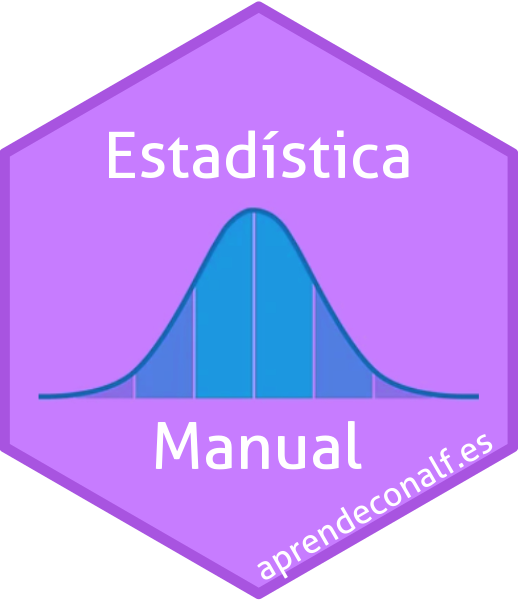
\includegraphics[width=0.4\textwidth]{img/logos/sticker.png}
\end{center}

\vfill

\begin{flushleft}
\begin{tabular}{ll}

\includegraphics[width=0.1\textwidth]{img/logos/aprendeconalf.png} & \parbox[b]{5cm}{\Large\textsf{Alfredo
Sánchez
Alberca}\\ \textsf{asalber@ceu.es} \\ \textsf{https://aprendeconalf.es}}
\end{tabular}
\end{flushleft}
\end{titlepage}
\renewcommand*\contentsname{Tabla de contenidos}
{
\hypersetup{linkcolor=}
\setcounter{tocdepth}{2}
\tableofcontents
}
\bookmarksetup{startatroot}

\chapter*{Prefacio}\label{prefacio}
\addcontentsline{toc}{chapter}{Prefacio}

\markboth{Prefacio}{Prefacio}

Colección de problemas de Bioestadística para el Master en
Nutrigenómica.

\bookmarksetup{startatroot}

\chapter{Contrastes de hipótesis
paramétricos}\label{contrastes-de-hipuxf3tesis-paramuxe9tricos}

\begin{exercise}[]\protect\hypertarget{exr-contraste-media-consumo-azucar}{}\label{exr-contraste-media-consumo-azucar}

Sabiendo que el año pasado el consumo per cápita de azúcar en España fue
de \(4.8\) kg y que este consumo sigue una distribución normal, hemos
seleccionado aleatoriamente a \(20\) españoles obteniendo una media
muestral de \(5\) kg y una cuasidesviación típica muestral de \(0.4\)
kg. Contrastar la hipótesis de que el consumo de azúcar per cápita de
este año en España no ha variado utilizando un nivel de significación
del \(10\)\%.

\end{exercise}

\begin{tcolorbox}[enhanced jigsaw, toprule=.15mm, breakable, opacityback=0, colback=white, coltitle=black, colbacktitle=quarto-callout-tip-color!10!white, toptitle=1mm, rightrule=.15mm, opacitybacktitle=0.6, leftrule=.75mm, colframe=quarto-callout-tip-color-frame, left=2mm, bottomtitle=1mm, titlerule=0mm, title=\textcolor{quarto-callout-tip-color}{\faLightbulb}\hspace{0.5em}{Solución}, arc=.35mm, bottomrule=.15mm]

Sea \(X\sim N(\mu,\sigma)\) la variable aleatoria que mide el consumo
per cápita de azúcar en España.\\
Número de poblaciones: 1 población. Variable dependiente: Consumo de
azúcar (cuantitativa).\\
Tamaño muestral: \(n=20\).\\
Contraste de la media de una población normal (prueba t):
\(H_0:\mu=4.8\), \(H_1:\mu\neq 4.8\).\\
Estadístico del contraste: \(t=2.24\)\\
p-valor: \(p =2 P(t(19)>2.24) = 0.037\).\\
Como el p-valor es menor que el nivel de significación \(\alpha = 0.1\),
se rechaza la hipótesis nula y se concluye que el consumo de azúcar per
cápita de este año en España ha variado.

\end{tcolorbox}

\begin{exercise}[]\protect\hypertarget{exr-contraste-proporcion-asistencia-clase}{}\label{exr-contraste-proporcion-asistencia-clase}

En una clase de alumnos de primaria se ha comprobado que el \(20\)\% del
alumnado consume bollería industrial. Para disminuir esta preocupante
cifra, el colegio ha implantado un programa de educación nutricional.
Después del programa se tomó una muestra aleatoria de \(50\) alumnos de
primaria y se observó que 8 seguían consumiendo bollería industrial.
Contrastar con un nivel de significación del \(5\)\% si el programa es
efectivo.

\end{exercise}

\begin{tcolorbox}[enhanced jigsaw, toprule=.15mm, breakable, opacityback=0, colback=white, coltitle=black, colbacktitle=quarto-callout-tip-color!10!white, toptitle=1mm, rightrule=.15mm, opacitybacktitle=0.6, leftrule=.75mm, colframe=quarto-callout-tip-color-frame, left=2mm, bottomtitle=1mm, titlerule=0mm, title=\textcolor{quarto-callout-tip-color}{\faLightbulb}\hspace{0.5em}{Solución}, arc=.35mm, bottomrule=.15mm]

Número de poblaciones: 1 población.\\
Variable dependiente: Consumo de bollería industrial (cualitativa
binaria).\\
Tamaño muestral: \(n=50\).\\
Contraste para la proporción de una población: \(H_0:p=0.2\),
\(H_1:p< 0.2\).\\
p-valor: \(p=0.2979\).\\
Como el p-valor es mayor que el nivel de significación
\(\alpha = 0.05\), no se rechaza la hipótesis nula y se concluye que no
hay evidencias significativas de que el programa sea efectivo.

\end{tcolorbox}

\begin{exercise}[]\protect\hypertarget{exr-contraste-media-consumo}{}\label{exr-contraste-media-consumo}

Se sabe que el consumo anual de helado correspondiente a cada español
sigue una distribución normal y que el año pasado el consumo medio fue
de 20 kg. Queremos contrastar si este año se va a mantener el consumo
medio de helado que el año pasado, y para comprobarlo se efectúa una
muestra aleatoria de 22 españoles, obteniéndose los resultados recogidos
en el fichero \href{datos/consumo-helado.csv}{consumo-helado.csv}.
Realizar el contraste con un nivel de significación de \(0.10\).

\end{exercise}

\begin{tcolorbox}[enhanced jigsaw, toprule=.15mm, breakable, opacityback=0, colback=white, coltitle=black, colbacktitle=quarto-callout-tip-color!10!white, toptitle=1mm, rightrule=.15mm, opacitybacktitle=0.6, leftrule=.75mm, colframe=quarto-callout-tip-color-frame, left=2mm, bottomtitle=1mm, titlerule=0mm, title=\textcolor{quarto-callout-tip-color}{\faLightbulb}\hspace{0.5em}{Solución}, arc=.35mm, bottomrule=.15mm]

Número de poblaciones: 1 población.\\
Variable dependiente: Consumo de helado (cuantitativa).\\
Tamaño muestral: \(n=22\).\\
Prueba de normalidad de Kolmogorov-Smirnov. p-valor: \(p=0.632\). Se
acepta la normalidad.\\
Contraste de la media de una población normal (prueba t):
\(H_0:\mu=20\), \(H_1:\mu\neq 20\).\\
p-valor: \(p = 0.8033\).\\
Como el p-valor es mayor que el nivel de significación
\(\alpha = 0.10\), no se rechaza la hipótesis nula y se concluye que el
consumo medio de helado de este año en España se va a mantener.

\end{tcolorbox}

\begin{exercise}[]\protect\hypertarget{exr-contraste-comparacion-medias-pareadas-hierro}{}\label{exr-contraste-comparacion-medias-pareadas-hierro}

Se ha realizado un estudio para comparar los niveles de hierro en sangre
antes y después de un programa de ejercicios. Los datos del estudio
están en el fichero
\href{datos/niveles-hierro-tratamiento.csv}{niveles-hierro-ejercicio.csv}.
Realizar el contraste de hipótesis adecuado para ver si el ejercicio
aumenta el nivel de hierro con un nivel de significación del 1\%.

\end{exercise}

\begin{tcolorbox}[enhanced jigsaw, toprule=.15mm, breakable, opacityback=0, colback=white, coltitle=black, colbacktitle=quarto-callout-tip-color!10!white, toptitle=1mm, rightrule=.15mm, opacitybacktitle=0.6, leftrule=.75mm, colframe=quarto-callout-tip-color-frame, left=2mm, bottomtitle=1mm, titlerule=0mm, title=\textcolor{quarto-callout-tip-color}{\faLightbulb}\hspace{0.5em}{Solución}, arc=.35mm, bottomrule=.15mm]

Número de poblaciones: 2 poblaciones pareadas (población 1: antes de
hacer ejercicio, población 2: después de hacer ejercicio).\\
Variable dependiente: Nivel de hierro (cuantitativa).\\
Tamaño muestral: \(n=20\).\\
Prueba de normalidad de Kolmogorov-Smirnov: p-valor de la diferencia:
\(0.804\). Se acepta la normalidad.\\
Contraste para la comparación de medias de poblaciones pareadas:
\(H_0:\mu_d=0\), \(H_1:\mu_d< 0\).\\
p-valor: \(p=0.0011\).\\
Como el p-valor es menor que el nivel de significación se rechaza la
hipótesis nula y se concluye que el programa de ejercicios ha aumentado
significativamente el nivel de hierro en sangre.

\end{tcolorbox}

\begin{exercise}[]\protect\hypertarget{exr-contraste-comparacion-medias-glucosa}{}\label{exr-contraste-comparacion-medias-glucosa}

Se ha realizado un estudio para comparar los niveles de glucosa en
sangre de dos grupos: uno sigue una dieta baja en carbohidratos y otro
una dieta estándar. Los datos del estudio están en el fichero
\href{datos/niveles-glucosa-dietas.csv}{niveles-glucosa-dietas.csv}.
Realizar el contraste de hipótesis adecuado para comparar las medias de
los dos grupos con un nivel de significación del 5\%.

\end{exercise}

\begin{tcolorbox}[enhanced jigsaw, toprule=.15mm, breakable, opacityback=0, colback=white, coltitle=black, colbacktitle=quarto-callout-tip-color!10!white, toptitle=1mm, rightrule=.15mm, opacitybacktitle=0.6, leftrule=.75mm, colframe=quarto-callout-tip-color-frame, left=2mm, bottomtitle=1mm, titlerule=0mm, title=\textcolor{quarto-callout-tip-color}{\faLightbulb}\hspace{0.5em}{Solución}, arc=.35mm, bottomrule=.15mm]

Número de poblaciones: 2 poblaciones independientes (población 1: dieta
baja en carbohidratos, población 2: dieta estándar).\\
Variable dependiente: Nivel de glucosa (cuantitativa).\\
Tamaños muestrales: \(n_1=30\), \(n_2=30\).\\
Contraste de comparación de varianzas: \(H_0:\sigma_1^2=\sigma_2^2\),
\(H_1:\sigma_1^2\neq \sigma_2^2\). p-valor: \(p=0.25\). Se acepta la
hipótesis nula de igualdad de varianzas.\\
Contraste para la comparación de medias de poblaciones independientes
con varianzas iguales: \(H_0:\mu_1=\mu_2\), \(H_1:\mu_1<\mu_2\).\\
p-valor: \(p=0.00009\). Como el p-valor es menor que el nivel de
significación se rechaza la hipótesis nula y se concluye que el nivel de
glucosa en sangre es significativamente menor en el grupo que sigue una
dieta baja en carbohidratos.

\end{tcolorbox}

\begin{exercise}[]\protect\hypertarget{exr-contraste-comparacion-medias-expresion-genica}{}\label{exr-contraste-comparacion-medias-expresion-genica}

Se ha realizado un estudio para comparar los niveles de expresión de un
gen en función de la dieta (vegetariana u omnívora). Los datos del
estudio están en el fichero
\href{datos/expresion-genica-dietas.csv}{expresion-genica-dietas.csv}.
Realizar el contraste de hipótesis adecuado para comparar las medias de
los dos grupos.

\end{exercise}

\begin{tcolorbox}[enhanced jigsaw, toprule=.15mm, breakable, opacityback=0, colback=white, coltitle=black, colbacktitle=quarto-callout-tip-color!10!white, toptitle=1mm, rightrule=.15mm, opacitybacktitle=0.6, leftrule=.75mm, colframe=quarto-callout-tip-color-frame, left=2mm, bottomtitle=1mm, titlerule=0mm, title=\textcolor{quarto-callout-tip-color}{\faLightbulb}\hspace{0.5em}{Solución}, arc=.35mm, bottomrule=.15mm]

Número de poblaciones: 2 poblaciones independientes (población 1: dieta
vegetariana, población 2: dieta omnívora).\\
Variable dependiente: Expresión génica (cuantitativa).\\
Tamaños muestrales: \(n_1=20\), \(n_2=25\).\\
Prueba de normalidad de Kolmogorov-Smirnov: p-valor primera muestra:
\(0.4164\), p-valor segunda muestra: \(0.2767\). Se acepta la normalidad
en ambos grupos.\\
Contraste de comparación de varianzas: \(H_0:\sigma_1^2=\sigma_2^2\),
\(H_1:\sigma_1^2\neq \sigma_2^2\). p-valor: \(p=0.1373\). Se acepta la
hipótesis nula de igualdad de varianzas.\\
Contraste para la comparación de medias de poblaciones independientes
con varianzas iguales: \(H_0:\mu_1=\mu_2\), \(H_1:\mu_1<\mu_2\).\\
p-valor: \(p=0.00006\).\\
Como el p-valor es menor que el nivel de significación, se rechaza la
hipótesis nula y se concluye que existen diferencias estadísticamente
significativas en los niveles de expresión génica en función de la
dieta.

\end{tcolorbox}

\begin{exercise}[]\protect\hypertarget{exr-contraste-comparacion-proporciones-vitamina-c}{}\label{exr-contraste-comparacion-proporciones-vitamina-c}

Se utiliza un grupo de 150 pacientes para comprobar la teoría de que la
vitamina C tiene alguna influencia en el tratamiento del cáncer. Los 150
pacientes fueron divididos en dos grupos de 75. Un grupo recibió 10
gramos de vitamina C y el otro un placebo cada día, además de la
medicación habitual. De los que recibieron la vitamina C, 47 presentaban
alguna mejoría al cabo de cuatro semanas, mientras que de los que
recibieron el placebo, 43 experimentaron mejoría. Contrastar la
hipótesis de que la vitamina C tiene influencia en el tratamiento del
cáncer con un nivel de significación del 5\%.

\end{exercise}

\begin{tcolorbox}[enhanced jigsaw, toprule=.15mm, breakable, opacityback=0, colback=white, coltitle=black, colbacktitle=quarto-callout-tip-color!10!white, toptitle=1mm, rightrule=.15mm, opacitybacktitle=0.6, leftrule=.75mm, colframe=quarto-callout-tip-color-frame, left=2mm, bottomtitle=1mm, titlerule=0mm, title=\textcolor{quarto-callout-tip-color}{\faLightbulb}\hspace{0.5em}{Solución}, arc=.35mm, bottomrule=.15mm]

Número de poblaciones: 2 poblaciones independientes (población 1:
vitamina C, población 2: placebo).\\
Variable dependiente: Mejoría en el tratamiento del cáncer (cualitativa
binaria).\\
Tamaños muestrales: \(n_1=75\), \(n_2=75\).\\
Contraste para la comparación de proporciones: \(H_0:p_1=p_2\),
\(H_1:p_1\neq p_2\).\\
p-valor: \(p=0.6824\).\\
Como el p-valor es mayor que el nivel de significación, no se rechaza la
hipótesis nula y se concluye que no hay evidencias significativas de que
la vitamina C tenga influencia en el tratamiento del cáncer.

\end{tcolorbox}

\begin{exercise}[]\protect\hypertarget{exr-contraste-proporcion-consumo-alcohol}{}\label{exr-contraste-proporcion-consumo-alcohol}

En un estudio sobre el consumo de alcohol entre los jóvenes durante los
fines de semana, se preguntó a 100 chicos y a 125 chicas, de los que 63
chicos y 59 chicas contestaron que consumían. En vista de estos datos,
¿existe alguna diferencia significativa entre las proporciones de chicos
y chicas que consumen alcohol los fines de semana?

\end{exercise}

\begin{tcolorbox}[enhanced jigsaw, toprule=.15mm, breakable, opacityback=0, colback=white, coltitle=black, colbacktitle=quarto-callout-tip-color!10!white, toptitle=1mm, rightrule=.15mm, opacitybacktitle=0.6, leftrule=.75mm, colframe=quarto-callout-tip-color-frame, left=2mm, bottomtitle=1mm, titlerule=0mm, title=\textcolor{quarto-callout-tip-color}{\faLightbulb}\hspace{0.5em}{Solución}, arc=.35mm, bottomrule=.15mm]

Número de poblaciones: 2 poblaciones independientes (población 1:
chicos, población 2: chicas).\\
Variable dependiente: Consumo de alcohol (cualitativa binaria).\\
Tamaños muestrales: \(n_1=100\), \(n_2=125\).\\
Contraste para la comparación de proporciones: \(H_0:p_1=p_2\),
\(H_1:p_1\neq p_2\).\\
p-valor: \(p=0.0163\).\\
Como el p-valor es menor que el nivel de significación, se rechaza la
hipótesis nula y se concluye que hay diferencias significativas entre el
consumo de alcohol de chicos y chicas.

\end{tcolorbox}



\end{document}
